% !TEX root = MAIN.tex

\section{SEMuS}

The activity \emph{Execute FAQAS-CompileAndExecuteMutants} in Figure~\ref{fig:process:codeDriven:augmentation} concerns the execution of the program \emph{FAQAS-GenerateTestGenerationScaffolding}.

\begin{figure}[h]
  \centering
	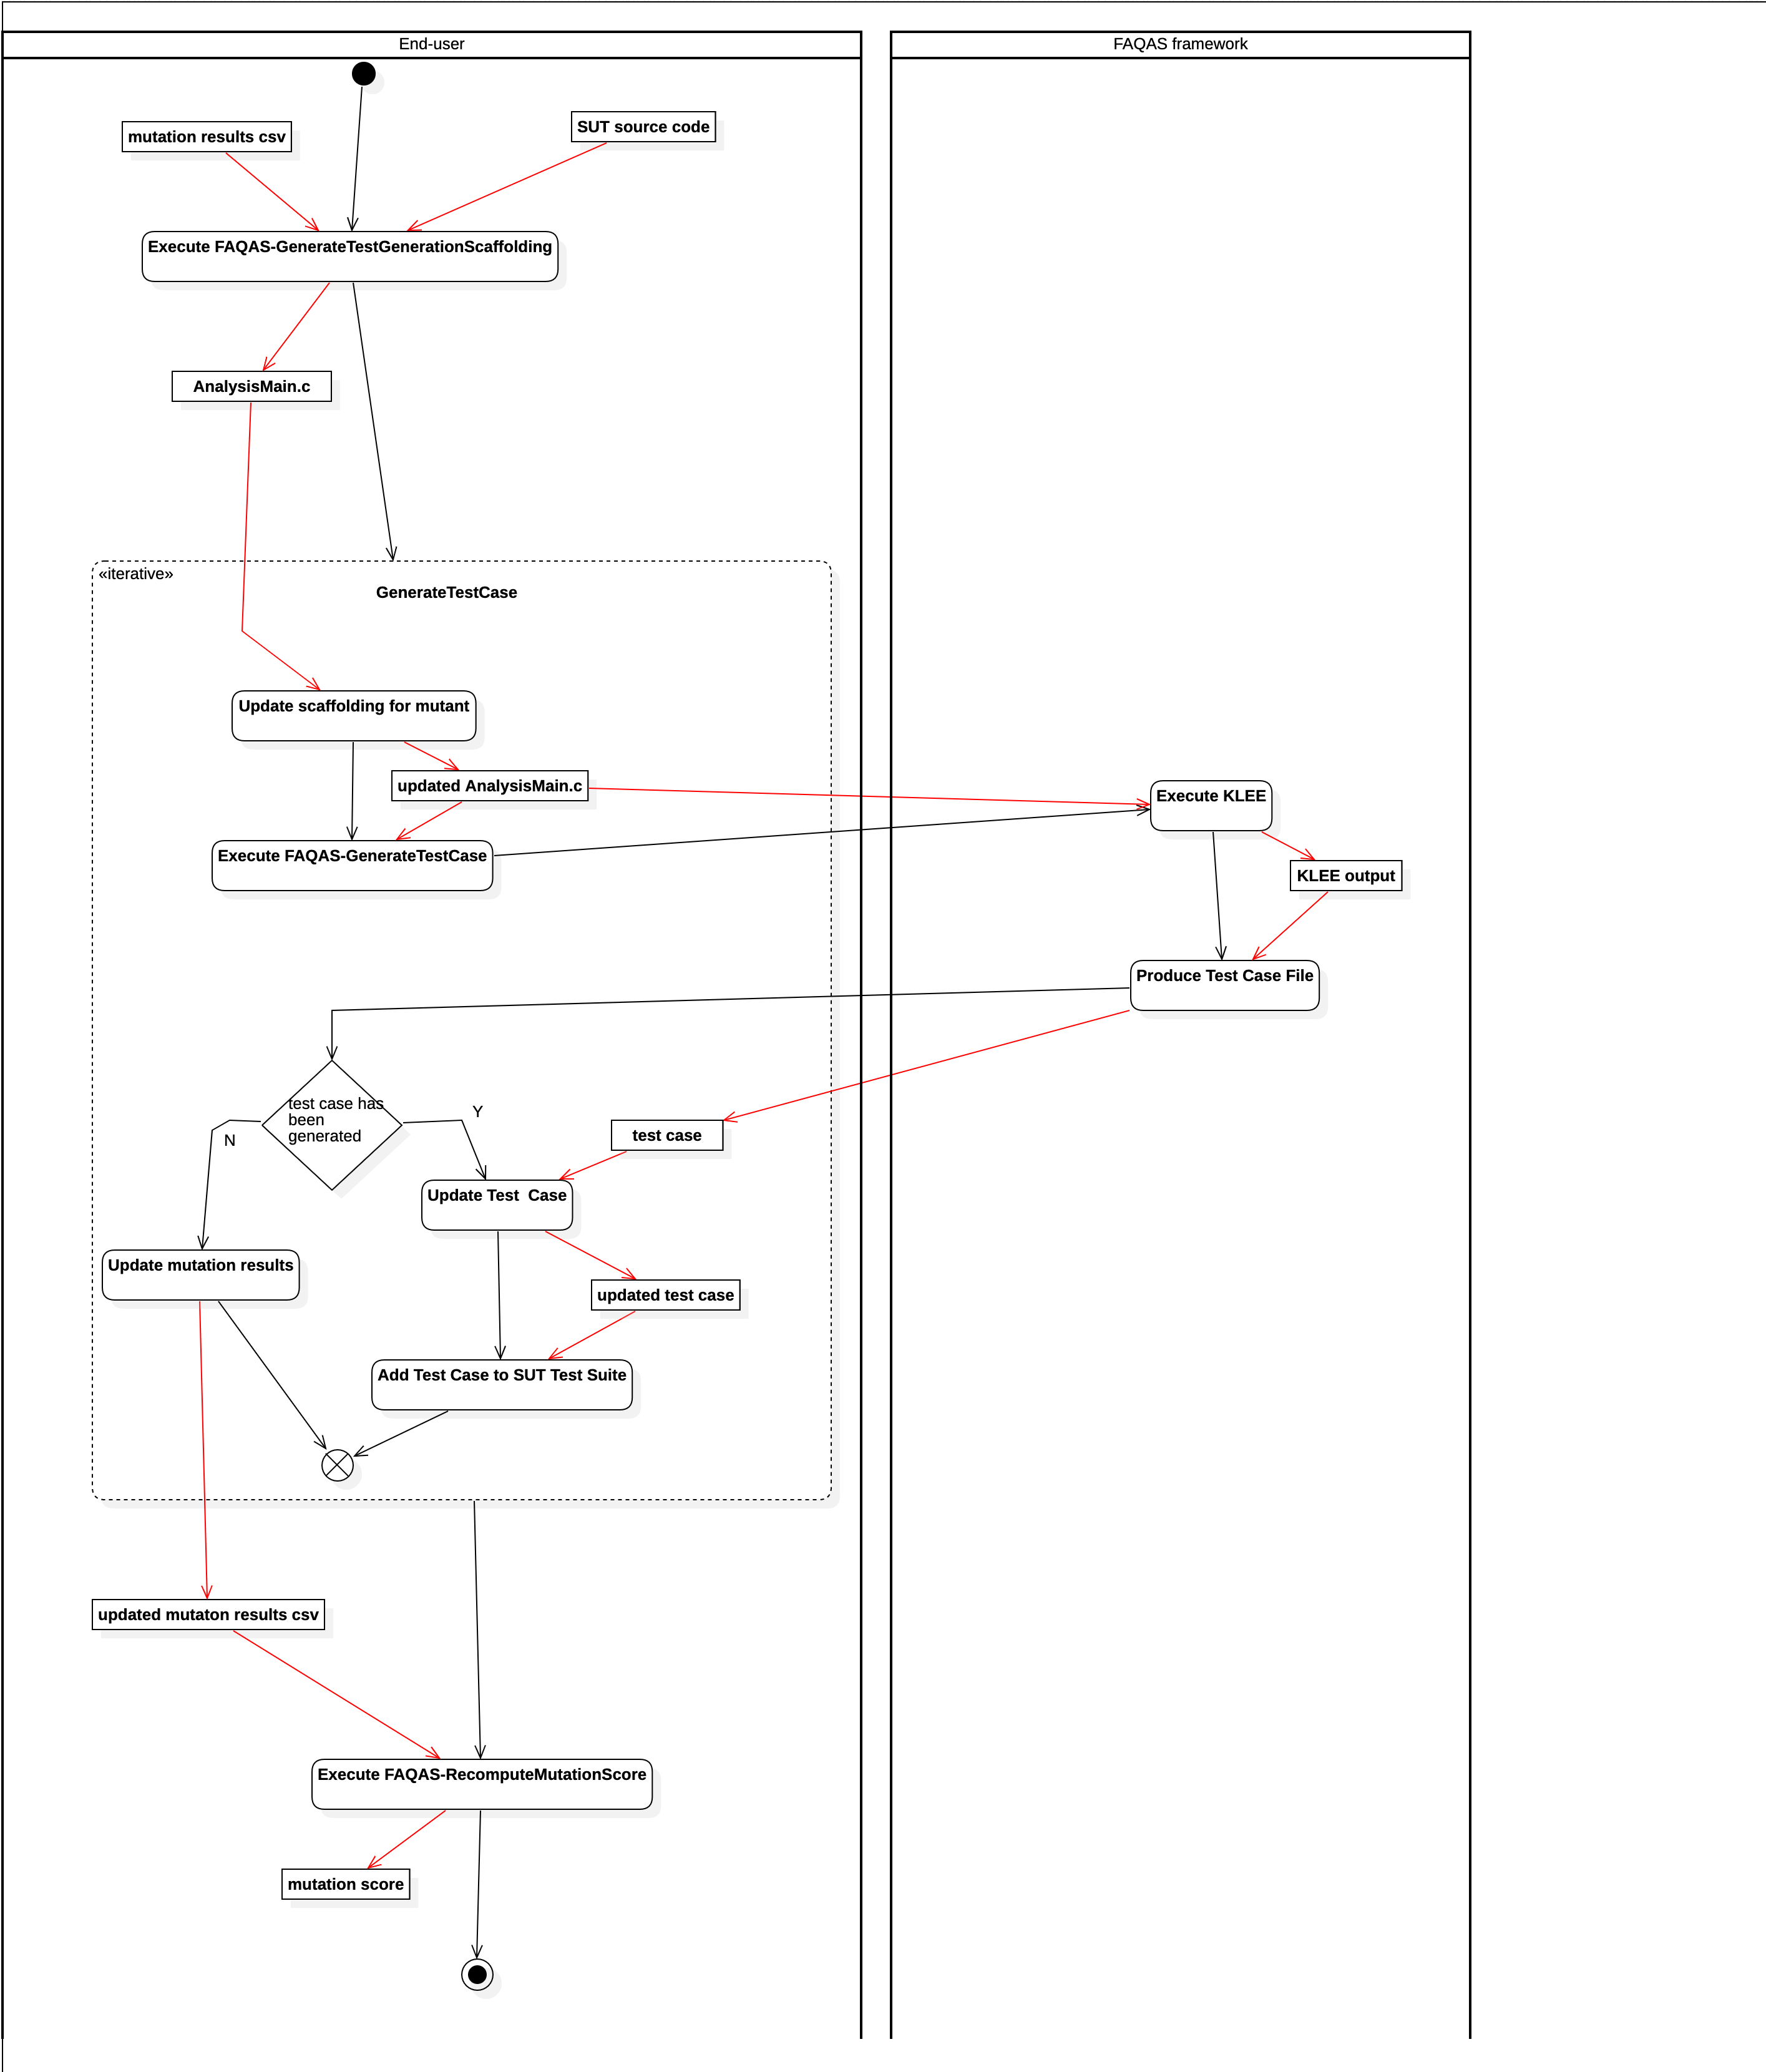
\includegraphics[width=\textwidth]{images/png/Activity1!CodeDrivenTestSuiteAugmentation_2.png}
      \caption{Overview of the code-driven test suite augmentation process.}
      \label{fig:process:codeDriven:augmentation}
\end{figure}

The code-driven mutation testing component also implements the process for the improvement of the effectiveness of test suites that is drafted in Figure~\ref{fig:process:codeDriven:augmentation}. Figure~\ref{fig:process:codeDriven:augmentation} relies on UML activity diagram notation. In Figure~\ref{fig:process:codeDriven:augmentation} the execution of specific software artefacts from the end user is made explicit. Also, we use black arrows to draw control-flow, red arrows for data-flow.

The program \emph{FAQAS-GenerateTestGenerationScaffolding} takes as input the path of the \emph{SUT source code} and the file \emph{mutation results csv}. It generates a number of files named \emph{MutantId\_AnalysisMain.c}, one for each live mutant, where MutantId is the ID of a mutant. The file \emph{MutantId\_AnalysisMain.c} contains a main function that should be used for the analysis with KLEE. 

The content of file \emph{MutantId\_AnalysisMain.c} should resemble \emph{Listing 1.7} and \emph{Listing 1.9} of D2, it should enable the analysis with KLEE. For example, it should import the source file with the original function targeted by the mutation and the source code of the mutated function. Also, it should contain the definition of all the variables used for the execution of KLEE and a tentative set of required assertions.

The activity \emph{Update scaffolding for mutant} in Figure~\ref{fig:process:codeDriven:augmentation} indicates that the engineer should modify the file  \emph{MutantId\_AnalysisMain.c} if necessary. In particular, it might be necessary to refine the assertions produced by \emph{FAQAS-GenerateTestGenerationScaffolding}. More precisely, since assertions should concern output variables, it is necessary to verify that all the necessary output variables had been referred in assertion. Indeed, in C, with pointers and pointers to pointers, it is not possible to have a precise automated identification of output variables.

The activities in the expansion region \emph{generateTestCase} are repeated for every live mutant.

The activity \emph{Execute FAQAS-GenerateTestCase} in Figure~\ref{fig:process:codeDriven:augmentation} concerns the execution of the program \emph{FAQAS-GenerateTestCase}.

The program \emph{FAQAS-GenerateTestCase} generates a tentative unit test case (i.e., a source file in C) that kills the mutant. It executes the KLEE program and then produces a unit test case (i.e., a file with a main in C) after processing the KLEE output.

For test generation, the support for the programming language of the SUT depends on KLEE (it supports C, limited support for C++).

The test case generated by \emph{FAQAS-GenerateTestCase} contains an invocation of the function under test (i.e., the function targeted  by the mutation) along with assigned arguments and an assertion that verifies results. The values for the assigned arguments and the verification of results are derived from the output of KLEE.

If the program \emph{FAQAS-GenerateTestCase} successfully generates a test case, the engineer proceeds with inspecting it (activity \emph{Update Test  Case}), otherwise he can consider the mutant as equivalent (activity \emph{Update mutation results}).

The activity \emph{Update Test  Case} in Figure~\ref{fig:process:codeDriven:augmentation} is performed by the engineer. He may need to execute the generated test case to verify that KLEE has generated valid inputs (e.g., inputs that meet the program preconditions). Based on KLEE results, \emph{FAQAS-GenerateTestCase} also generates assertions that reflect the output observed by KLEE (e.g., \texttt{assert( output == value\_observed\_by\_KLEE)} ). The engineer should thus also verify that the assertion with the expected value is correct (i.e., it reflects what indicated in the SUT specifications). If the value appearing in the assertion is not correct, it means that KLEE during its execution has observed an incorrect value being generated by the SUT; for this reason, the SUT might be faulty and should be fixed.

The activity \emph{Add Test Case to SUT Test Suite} in Figure~\ref{fig:process:codeDriven:augmentation} is performed by the engineer, who may add the new test case to the test suite.

The activity \emph{Update mutation results} in Figure~\ref{fig:process:codeDriven:augmentation} is performed when a test case is not generated. This generally happens when the mutant cannot be killed (i.e., is equivalent). The engineer is expected to manually inspect the mutant to be sure that the mutant is equivalent (otherwise the missing test case is due to a limitation of KLEE). If the mutant is equivalent the engineer removes it from the file \emph{mutation results csv}.

The activity \emph{Execute FAQAS-RecomputeMutationScore} in Figure~\ref{fig:process:codeDriven:augmentation}  concerns the execution of the program \emph{FAQAS-RecomputeMutationScore}. It is performed after generating test cases for all the live mutants. Program \emph{FAQAS-RecomputeMutationScore} recomputes the mutation score after ignoring the equivalent mutants detected by KLEE.



